\chapter{P公司小微贷款业务服务质量现状与问题诊断}

本章以DMAIC方法论的界定阶段（Define）为主线，系统呈现P公司小微贷款业务的运营全貌、服务流程、服务质量现状数据，并在此基础上识别关键问题，明确后续改进项目的边界与目标。全章数据均来源于P公司内部运营系统、客户投诉记录及初步客户满意度摸底调查。\par

\section{3.1 P公司及小微贷款业务概况}

P公司是一家持牌普惠金融公司，属于非银行金融机构，专注于为小微企业和个体工商户提供经营性贷款服务。近年来，国家持续推进普惠金融政策落地，数字普惠金融的发展也为中小微企业的融资可得性提供了新的支撑\cite{ref7,ref2}。在此背景下，P公司逐步建立了覆盖多省域、多产品线的业务体系。\par

截至分析时点，P公司业务已覆盖5个省份、28个城市，形成了较为稳定的区域服务网络（数据来源：P公司内部运营系统）。公司目前运营3条小微贷款产品线：一是信用贷款产品，授信额度为10万元至100万元，面向经营稳定、征信良好的小微客户；二是担保贷款产品，授信额度为50万元至300万元，适用于能够提供合格担保措施的企业；三是供应链贷款产品，授信额度为30万元至500万元，依托核心企业信用向其上下游小微主体提供融资。三条产品线覆盖了不同资产规模和经营阶段的小微客户需求。\par

在服务渠道方面，P公司形成了线上线下融合的服务体系。线上渠道（App和小程序）承载了约55\%的业务量，客户可以自助完成产品浏览、额度测算和申请提交；客户经理线下服务承接约35\%的业务，通过面对面沟通为客户提供方案咨询和材料指导；另有约10\%的业务经由合作渠道引荐。公司当前活跃贷款客户约3,200户，贷款余额约18亿元。一线客户经理团队约45人，人均管户约70户（数据来源：P公司内部业务系统数据）。从人均管户数量来看，客户经理的工作负荷已处于较高水平，服务质量面临压力。\par

\section{3.2 小微贷款业务服务流程}

P公司小微贷款业务从客户接触到贷款结清，可归纳为七个核心服务环节，各环节的服务质量直接影响客户的整体感知。参考张小敏\cite{ref11}对小微线上贷款流程的优化研究以及李欣春\cite{ref55}对普惠信贷客户触达的分析，本文梳理了P公司完整的服务流程链路，并标注了每个环节存在的服务质量痛点。\par

\begin{table}[htbp]
  \centering
  \small
  \caption{P公司小微贷款业务服务流程与服务质量痛点}
  \resizebox{\textwidth}{!}{%
  \begin{tabular}{p{1.8cm} p{1.2cm} p{1.2cm} p{1.2cm} p{6.6cm}}
    \toprule
    \textbf{环节} & \textbf{标准时效} & \textbf{实际中位数} & \textbf{一次通过率} & \textbf{客户接触点与服务质量痛点} \\
    \midrule
    获客触达 & —— & —— & —— & 线上广告投放、客户经理外呼、存量客户转介；痛点：信息不对称，客户对产品条件和费用结构缺乏事前了解 \\
    申请提交 & 即时 & 即时 & —— & App或小程序自助填写、客户经理线下协助填表；痛点：线上线下存在断点，App端申请后仍需补交纸质材料 \\
    资料审核与补正 & 2工作日 & 4.5工作日 & 62\% & 风控系统初审后，通过短信或电话通知客户补充材料；痛点：补正要求表述笼统（如"材料不齐全"），客户平均补正1.8次，补正率达28\% \\
    授信审批 & 7工作日 & 12工作日 & 72\% & 审批进度仅能被动等待通知，客户无法自主查询；痛点：审批超时严重，进度不透明，客户产生焦虑 \\
    签约放款 & 1工作日 & 2工作日 & 95\% & 电子签约平台完成合同签署，系统自动发起放款并发送到账通知；该环节相对顺畅 \\
    贷后管理 & 按季回访 & 实际半年1次 & —— & 客户经理通过电话或短信进行贷后回访；痛点：回访频率显著低于标准要求，客户经营变化难以及时发现 \\
    投诉处理 & 5工作日闭环 & 7工作日 & 62\%闭环率 & 客户可通过客服热线或线上工单提交投诉；痛点：闭环率偏低，23\%的投诉为重复投诉，缺乏根因回溯机制 \\
    \bottomrule
  \end{tabular}%
  }
\end{table}

从流程数据可以清晰看出，资料审核与补正、授信审批以及投诉处理是三个服务时效偏离标准最为突出的环节。其中，授信审批的实际耗时（12个工作日）接近承诺标准（7个工作日）的两倍，资料补正环节的一次通过率仅为62\%，意味着超过三分之一的申请需要客户反复补充材料，严重影响服务体验。\par

\begin{figure}[htbp]
  \centering
  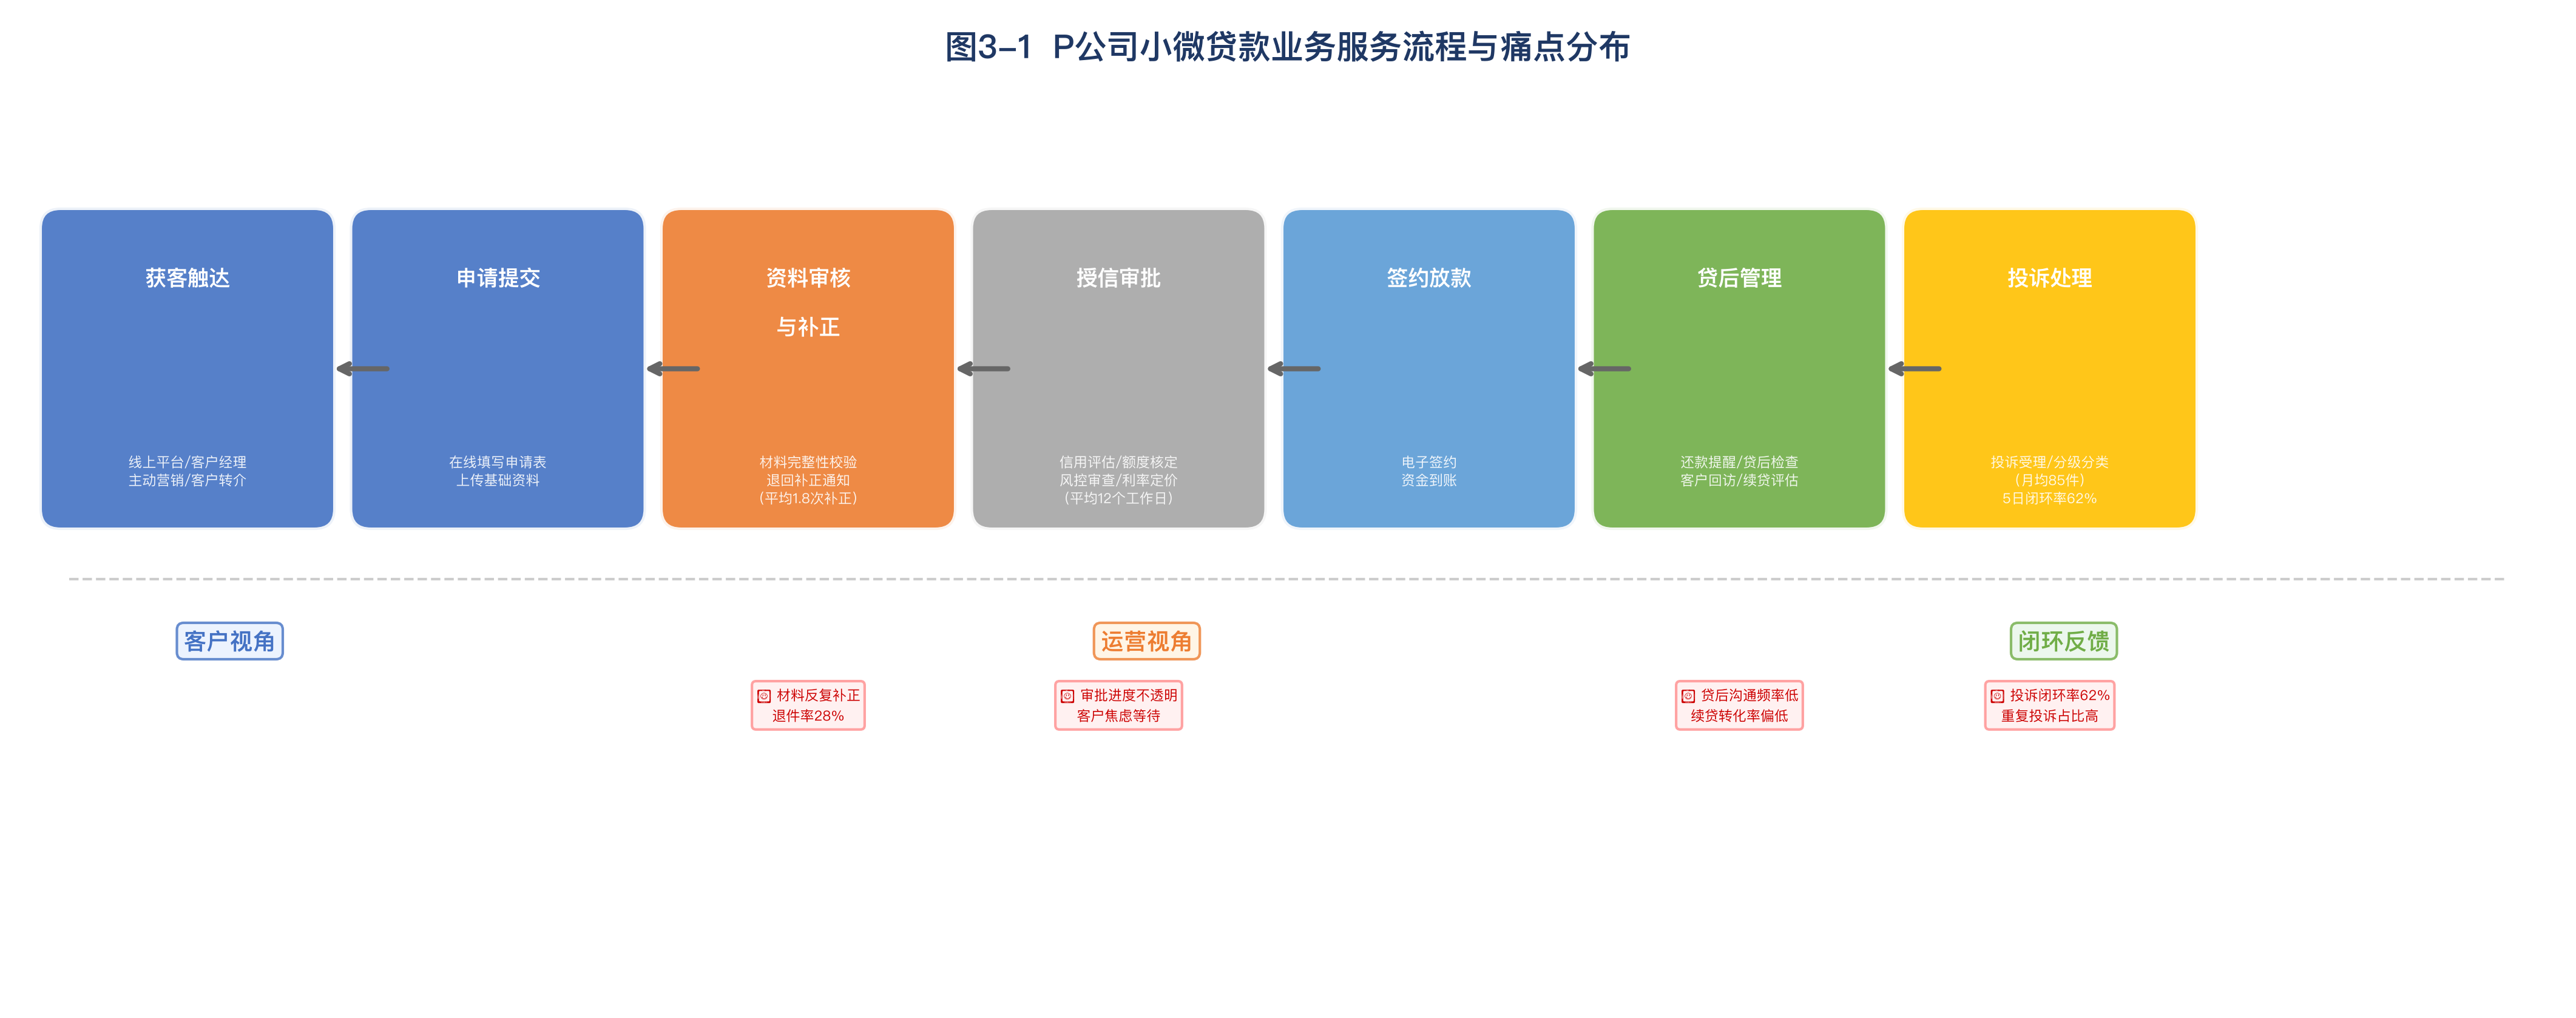
\includegraphics[width=\textwidth]{figures/图3-1_P公司服务流程图.png}
  \caption{P公司小微贷款业务服务流程图}
  \label{fig:3-1}
\end{figure}

\section{3.3 服务质量现状数据}

为进一步量化P公司小微贷款业务的服务质量水平，本节将P公司内部运营数据脱敏后分析如下。参考花青青等\cite{ref15}在金融机构服务质量评价中的指标设计框架，选取了能够反映服务效率、服务准确性和客户反馈的核心指标。\par

\begin{table}[htbp]
  \centering
  \small
  \caption{P公司小微贷款业务服务质量核心指标（近12个月）}
  \resizebox{\textwidth}{!}{%
  \begin{tabular}{p{2.5cm} p{6cm} p{3.5cm}}
    \toprule
    \textbf{指标类别} & \textbf{指标名称} & \textbf{数值} \\
    \midrule
    业务规模 & 业务办理量 & 1,860笔 \\
    服务效率 & 平均办理时长（申请至放款） & 12个工作日（25分位数：5个工作日，75分位数：20个工作日） \\
    服务效率 & 材料补正率 & 28\%（平均每笔补正1.8次） \\
    服务准确性 & 一次通过率（资料无需补正） & 62\% \\
    服务准确性 & 退件率（补正后仍不通过） & 8\% \\
    客户反馈 & 投诉总量 & 1,024件，月均85件 \\
    客户反馈 & 投诉闭环率（5日内解决） & 62\% \\
    客户反馈 & 重复投诉率 & 23\% \\
    客户反馈 & 客户满意度初测（5分制） & 3.12 \\
    \bottomrule
  \end{tabular}%
  }
\end{table}

从数据可以看到，P公司小微贷款业务的服务质量在多个维度存在明显短板。平均办理时长12个工作日表明客户从提交申请到获得放款需要等待近三周，且个案差异极大（75分位数达20个工作日）。材料补正率28\%和一次通过率62\%相互印证，说明近四成客户的申请流程不顺畅。客户满意度初测仅3.12分（5分制），处于"基本满意"与"一般"之间的偏低区间，与行业标杆水平存在显著差距。\par

P公司客诉管理系统记录显示，投诉数据进一步揭示了客户不满的集中方向。对近12个月1,024件投诉的归类分析如下：\par

\begin{table}[htbp]
  \centering
  \small
  \caption{P公司小微贷款业务客户投诉类型分布}
  \resizebox{\textwidth}{!}{%
  \begin{tabular}{p{6cm} p{2cm} p{2cm}}
    \toprule
    \textbf{投诉类型} & \textbf{占比} & \textbf{件数} \\
    \midrule
    审批时效慢 & 32\% & 328 \\
    材料要求不清晰 & 22\% & 225 \\
    客户经理响应慢 & 18\% & 184 \\
    贷款方案不匹配 & 12\% & 123 \\
    贷后服务不足 & 8\% & 82 \\
    费用透明度不足 & 5\% & 51 \\
    其他 & 3\% & 31 \\
    \bottomrule
  \end{tabular}%
  }
\end{table}

审批时效慢和材料要求不清晰两项合计占总投诉量的54\%，是客户不满的首要来源。客户经理响应慢（18\%）和贷款方案不匹配（12\%）分列第三、第四位，反映出服务人员能力和产品设计层面的问题不容忽视。\par

\begin{figure}[htbp]
  \centering
  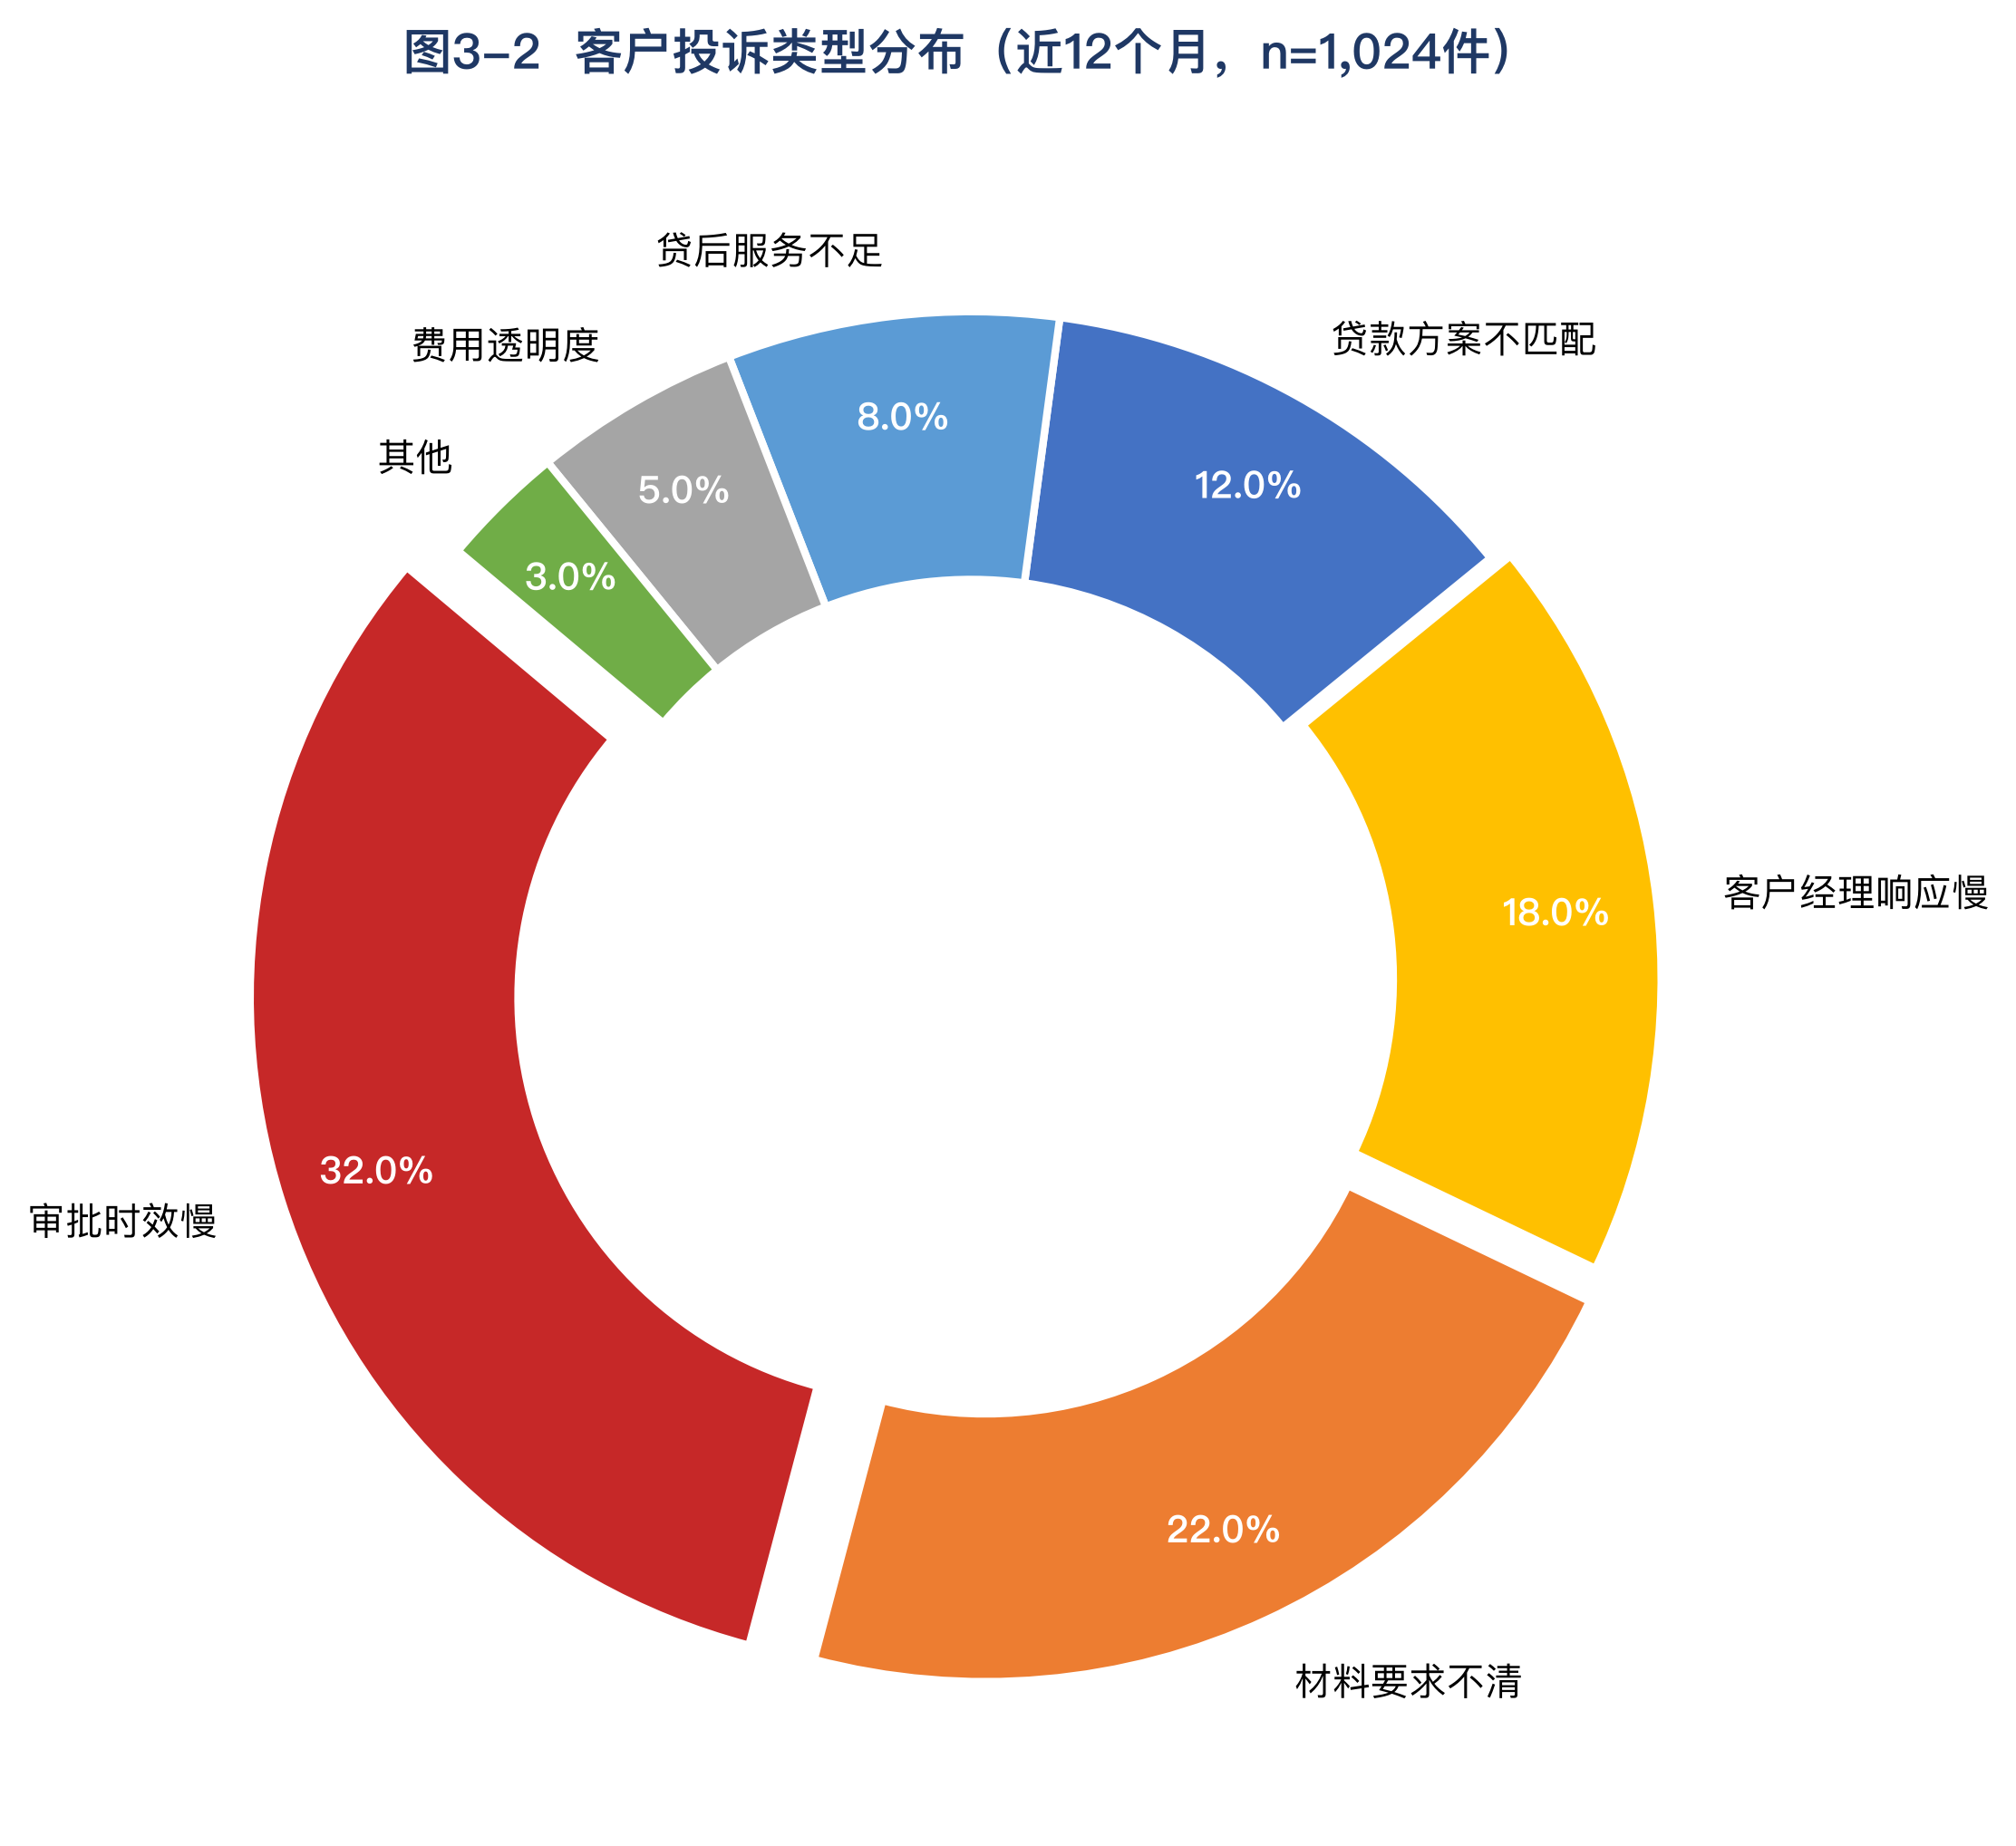
\includegraphics[width=\textwidth]{figures/图3-2_客户投诉类型分布.png}
  \caption{P公司小微贷款业务客户投诉类型分布}
  \label{fig:3-2}
\end{figure}

\section{3.4 主要服务质量问题识别}

基于上述流程分析和现状数据，本节借鉴Parasuraman等提出的SERVQUAL服务质量评价模型\cite{ref14}的维度框架，结合花青青等\cite{ref15}、孙彦佩\cite{ref37}和黄兆锟\cite{ref38}在金融机构服务质量诊断中的研究实践，从客户旅程视角对P公司小微贷款业务的主要服务质量问题进行系统识别。识别标准为：该问题在投诉数据中有明确占比支撑，或在流程数据中表现为显著偏离承诺标准。\par

\begin{table}[htbp]
  \centering
  \small
  \caption{P公司小微贷款业务主要服务质量问题清单}
  \resizebox{\textwidth}{!}{%
  \begin{tabular}{p{2.2cm} p{2.4cm} p{3.7cm} p{3.7cm}}
    \toprule
    \textbf{问题维度} & \textbf{对应SERVQUAL维度} & \textbf{具体表现} & \textbf{影响} \\
    \midrule
    响应速度慢 & 响应性（Responsiveness） & 授信审批平均耗时12个工作日，远超承诺的7个工作日；资料补正通知周期为4.5个工作日，超出标准2.3倍；客户经理回访频率仅为承诺的一半 & 客户等待焦虑加剧，部分客户因时效过长放弃申请或转向其他融资渠道，客户流失风险上升 \\
    信息不透明 & 透明性$\bigstar$（Transparency） & 审批进度不可实时查询，客户只能被动等待；退件原因表述笼统（如"材料不齐全""资质不符"），缺乏具体指向；费用构成未在事前充分说明 & 信息不透明导致客户反复补正（补正率28\%），增加客户时间成本和负面情绪，严重削弱客户对服务过程的信任 \\
    线上线下断点 & 便利性$\bigstar$（Convenience） & 客户通过App提交电子申请后，仍需线下提交纸质证明材料；线上与线下渠道的信息同步不及时，客户需要重复提供相同信息 & 全流程服务体验割裂，背离数字金融背景下客户对"一次办结"的合理期待，便利性感知显著下降 \\
    产品匹配弱 & 产品适配$\bigstar$（Product Fit） & 标准化产品方案难以灵活匹配不同经营规模、不同生命周期小微客户的差异化资金需求；续贷客户不能享受简化流程 & 客户满意度低、续贷意愿不足；12\%的投诉指向方案不匹配，反映出产品设计与客户实际需求之间存在结构性背离 \\
    客户经理能力参差 & 保证性（Assurance） & 新入职客户经理占比约40\%，对公司产品、政策和审批规则的掌握不够系统，不同客户经理对同一问题的答复口径不一致 & 客户感知到的专业性不足，信任度下降；18\%的投诉涉及客户经理响应慢，表明客户经理能力差距已直接转化为服务质量的显性问题 \\
    投诉闭环差 & 可靠性（Reliability） & 投诉闭环率仅62\%，近四成投诉未在承诺的5个工作日内得到有效解决；重复投诉率高达23\%；缺乏系统化的根因回溯与改进机制 & 同类问题反复发生，投诉处理停留在"个案化解"层面，未能从流程和管理层面消除问题根源，客户对服务可靠性的信心持续受损 \\
    \bottomrule
  \end{tabular}%
  }
  {\footnotesize 注：$\bigstar$标记的维度为针对小微贷款服务场景在经典SERVQUAL五维模型基础上扩展的新维度。}
\end{table}

上述六个问题维度覆盖了从客户首次接触到贷后管理的完整服务链条，相互之间存在关联放大效应。审批时效慢加剧了客户对信息透明的需求，而信息不透明又进一步导致客户反复补正材料，拉长了整体办理时长。客户经理能力参差与投诉闭环差之间也存在传导关系：一线服务能力的不足增加了投诉发生的概率，而投诉处理机制的不健全又使这些问题无法被及时发现和纠正。这些问题的深层原因在于P公司缺乏系统化的服务质量评价和管理机制，服务质量的改进仍停留在零散的、被动响应式的层面。\par

\section{3.5 改进项目边界和目标}

基于上述现状诊断，本文明确后续改进研究的工作边界（数据来源：P公司内部资料）。改进范围聚焦于P公司小微贷款业务的服务质量，不扩展至公司全部金融产品线，也不涉及公司战略、组织架构或信息系统的整体重构\cite{ref10}。\par

改进项目围绕六个核心维度设定目标：一是缩短办理时长，将平均申请至放款周期压缩至承诺标准以内；二是提升材料一次通过率，减少客户反复补正的摩擦成本；三是增强信息透明度，实现审批进度可查询、退件原因可追溯；四是提高投诉闭环率，建立从投诉受理到根因改进的闭环管理机制；五是提升客户满意度，通过服务质量的系统性改进推动满意度评分向行业优秀水平靠拢；六是巩固风险合规底线，确保服务提速不以牺牲风控质量为代价\cite{ref24}。\par

在风险控制方面，依照P公司内部制度文件规定，改进项目明确将不良贷款率控制在2.0\%以内作为硬性约束。服务质量改进的任何措施均需在满足该风控边界的前提下实施，不得以放松授信标准、简化风控流程或降低审批质量来换取服务时效的缩短\cite{ref24}。这一边界条件的设定确保了服务质量改进与风险管理的平衡，也是DMAIC方法中界定阶段确定项目约束的关键步骤。\par

综上所述，第3章通过P公司小微贷款业务的全景刻画、服务流程的系统梳理、服务质量现状数据的定量呈现以及主要问题的维度化识别，完成了DMAIC界定阶段的全部工作。上述诊断结果为第4章构建服务质量评价模型提供了明确的问题导向和实证基础。\par
